\documentclass[11pt]{article}
 
\usepackage[utf8]{inputenc}
\usepackage[T1]{fontenc}
\usepackage[english]{babel}
\usepackage{mathtools, bm}
\usepackage{amssymb, bm}
\usepackage{float}
\usepackage{makecell}

\usepackage{caption} % to center captions
\usepackage{subcaption} % subcaption for figures side by side

\usepackage{booktabs} % for super cool table
\usepackage[table,xcdraw]{xcolor}  % to put color in tables
\usepackage{tcolorbox} % add box
\usepackage{commath} % for absolute values

\usepackage[parfill]{parskip}
\usepackage{graphicx}
\usepackage{hyperref}
\usepackage[top=0.8in, bottom=0.8in, left=1in, right=1in]{geometry}
\usepackage{listings}
\usepackage{multirow}
\usepackage{titlesec}
\usepackage{titling}
\usepackage{amsmath}


\DeclareMathOperator*{\argmax}{arg\,max}
\DeclareMathOperator*{\argmin}{arg\,min}
\titlespacing*{\section}
{0pt}{0.3em}{0.3em}
\titlespacing*{\subsection}
{0pt}{0.2em}{0.2em}
\titlespacing*{\subsubsection}
{0pt}{0.1em}{0.1em}
\setlength{\droptitle}{-9em}

\renewcommand\thesubsection{\thesection.\arabic{subsection}} % Subsection starting with A, B, ...

\renewcommand\thefigure{\thesubsection.\arabic{figure}}

\newcommand{\horrule}[1]{\rule{\linewidth}{#1}} % Create horizontal rule command with 1 argument of height

\numberwithin{figure}{section} % to have per-section figure numbering

\title{	
\normalfont \normalsize 
\textsc{Master MVA \\
Deep Learning} \\ [12pt]
\horrule{0.5pt} \\[0.2cm] % Thin top horizontal rule
\textbf{TP 5}: Deep Learning for Natural Language Processing \\
\horrule{2pt} \\[0.3cm] % Thick bottom horizontal rule
}

\author{\texttt{victor.busa@ens-paris-saclay.fr}}
\date{}

\begin{document}
\maketitle

\section{Monolingual embeddings}
\section{Multilingual word embedddings}
\paragraph{Question} Using the orthogonality and the properties of the trace, prove that, for $X$ and $Y$ two matrices:

\begin{equation}
W^{\star} = \argmin\limits_{W \in O_d(\mathbb{R})} ||WX - Y||_F = UV^T \text{, with} \quad U \Sigma V^T = \text{SVD}(YX^T)
\end{equation}
\textbf{Answer}: We want to minimize $||WX - Y||_F$. Without loss of generality we can focus on minimizing $||WX - Y||_F^2$. Let $X,Y \in \mathbb{R}^(d \times n)$. We then have:

\begin{align*}
\min\limits_{W \in O_d(\mathbb{R})} &= Tr\left((WX)^T WX \right) - 2 Tr\left((WX)^T Y\right) + Tr(Y^TY) \\
&= Tr(X^TW^TWX) - 2 Tr(X^TW^TY) + Tr(Y^TY) \\
&= Tr(X^TX) + Tr(Y^TY) - 2Tr(YX^TW^T)
\end{align*}

Where we have used the fact that $W \in O_d(\mathbb{R})$, i.e $W^TW = I$. So finally we have that ($tr(X^TX) + Tr(Y^TY)$ being constant w.r.t $W$):

\begin{align*}
\min\limits_{W \in O_d(\mathbb{R})} ||WX - Y||_F &= \max\limits_{W \in O_d(\mathbb{R})} Tr(YX^TW^T) \\
&= \max\limits_{W \in O_d(\mathbb{R})} Tr(U \Sigma V^T W^T U)
\end{align*}

Where we have used the singular value decomposition of $YX^T$: $U \Sigma V^T = SVD(YX^T)$ \\

Now, as U, V, W are in $O_d(\mathbb{R})$, so their products $\widehat{W} = V^T W^T U$ is in $O_d(\mathbb{R})$ because $(O_d(\mathbb{R}), \times)$ is a group. \\

So finally, we have:

\begin{align*}
	\min\limits_{W \in O_d(\mathbb{R})} ||WX - Y||_F &= \max\limits_{W \in O_d(\mathbb{R})} Tr(YX^TW^T) \\
	&= \max\limits_{W \in O_d(\mathbb{R})} Tr(\Sigma \widehat{W}) \\
	&= \max\limits_{W \in O_d(\mathbb{R})} \sum\limits_{i = 0}^d \sigma_{ii} \widehat{w}_{ii}
\end{align*}

Where we have used the fact that $\Sigma$ is a diagonal matrix. So at the end to maximize the sum $\sum\limits_{i=0}^d \sigma_{ii} \widehat{w}_{ii}$, We should choose
$\widehat{W} = I_{d \times d}$ because $\widehat{W} \in O_d(\mathbb{R})$ and $\forall i \in \; [1,\hdots, d],\; \sigma_{ii} \geq 0$. \\

Hence: $\widehat{W} = V^T W^T U = I \Rightarrow W^T = V U^T \Rightarrow W = U V^T$

So, at the end we have that the maximum is attained for $W = UV^T$ where $U \Sigma V^T$ = SVD($YX^T$)

\section{Sentence classification with BoV}
\paragraph{Question} What is your training and dev errors using either the average of
word vectors or the weighted-average?

\textbf{Answer}: Quite weirdly we can see on table \ref{table:acc} that the logistic regression using mean average achieves a better accuracy on the testing
set then if we use the \emph{idf} average. Maybe it would have more sense to use a \emph{idf-tf} weighted average and not just an \emph{idf} weighted average.
\begin{table}[h]
\centering
\begin{tabular}{|c|c|c|}
\hline
\textbf{accuracy} & \textbf{mean average} & \textbf{idf average} \\ \hline
\textbf{Train} & 0.497 & 0.493 \\ \hline
\textbf{Test} & 0.447 & 0.415 \\ \hline
\end{tabular}
\caption{Accuracy on the Stanford Sentiment Treebank using logistic regression and a BoV with either mean average or idf weighted average}
\label{table:acc}
\end{table}

\textbf{Bonus question}: I have used the xgboost classifier as it usually leads to good results (cf Kaggle competition). Yet I wasn't able to achieve better results with it.

\section{Deep Learning model for classification}
\paragraph{Question} Which loss did you use? Write the mathematical expression of
the loss you used for the 5-class classification.

\textbf{Answer}: 
\begin{itemize}
\item This is a multi-class classification problem so I use a \textbf{categorical cross-entropy} loss function.
\item The mathematical expression is just (for 5 classes):
$$H(p, q) = - \sum\limits_{i=1}^5 y_i log(y_i')$$
where $y_i$ is the true probability distribution and $y_i'$ is the predicted probability
\end{itemize}

\paragraph{Question} Plot the evolution of train/dev results w.r.t the number of epochs. \\
\textbf{Answer}: the evolution of the train/dev results w.r.t the number of epochs is shown on Figure \ref{fig:graph_epoch}

\begin{figure}[H]
		\centering
		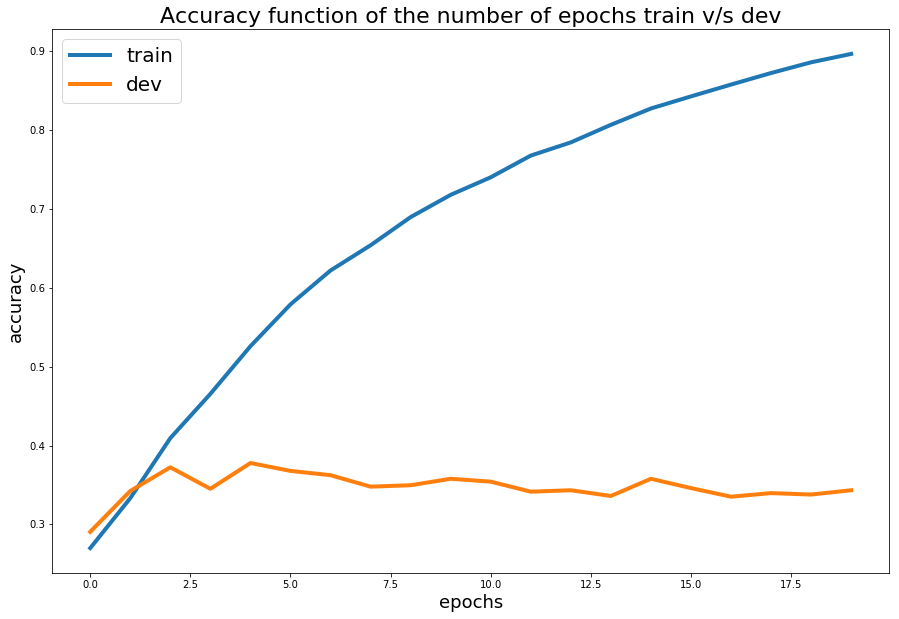
\includegraphics[width=1\linewidth]{images/graph_acc}
		\caption{Evolution of train and dev accuracy w.r.t the number of epochs}
		\label{fig:graph_epoch}
\end{figure}


\paragraph{Question} Be creative: use another encoder. What are your motivations for
using this other model?

We can use pretrained word-embeddings. The neural network will converge faster as it doesn't need to learn the word-embeddings from
scratch. At the end I have a better model. yet it is unable to achieve outstanding performance overall. Figure \ref{fig:graph_epoch2}
shows the evolution of the validation and training accuracy w.r.t to the number of epochs.

\begin{figure}[H]
		\centering
		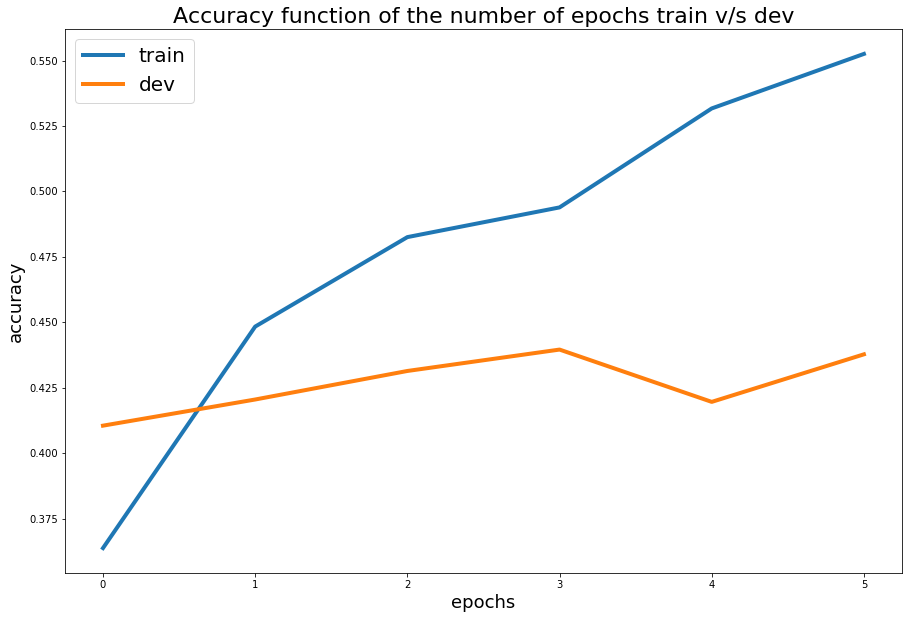
\includegraphics[width=1\linewidth]{images/graph_acc2}
		\caption{Evolution of train and dev accuracy w.r.t the number of epochs on the final model}
		\label{fig:graph_epoch2}
\end{figure}

\end{document}